	\chapter{Porównanie algorytmów}
	Jednym z algoytmów segmentacji chmur punktów 3D jest algorytm odległości Hausdorfa. Niniejszy projekt bazuje na nim, jednak zawiera pewne modyfikacje. Algorytm Hausdorfa grupuje punkty ze względu na ich odległości, oznaczając punkty jako obliczone i nieobliczone a także przypisując im odpowiednie numery grup.\cite{9286491}\\
	
	Warto jednak przedstawić ogólny podział metod segmentacji chmur punktów 3D. Przedstawiony został on na rysunku \ref{fig:segmethods}.\\%referencja że cho cho
	\\
	\begin{figure}[h!]
		\centering
		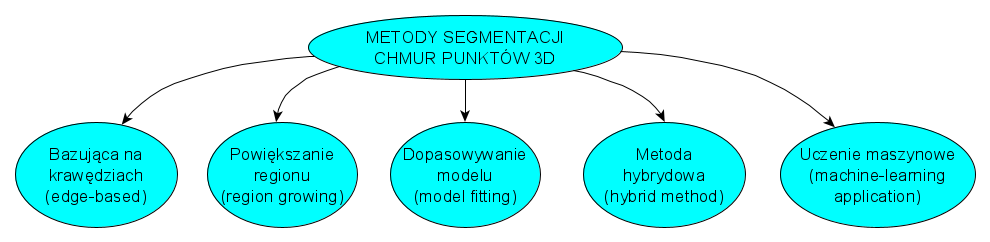
\includegraphics[width=\textwidth]{metody_segmentacji.png}
		\caption{Metody segmentacji}
		\label{fig:segmethods}
	\end{figure}
	\\%textbf żeby było ładniej
	\textbf{Metoda bazująca na krawędziach - }opiera się na wyodrębnieniu obszarów przy użyciu krawędzi i pogrupowaniu ich.\\
	\textbf{Powiększanie regionu - }metoda ta może zostać zaimplementowana w wersji z góry na dół lub z dołu w górę. Może też być połączeniem obu tych podejść. Metoda ta opiera się na wyodrębnieniu punktów o określonych cechach i pogrupowaniu ich.\\
	\textbf{Dopasowywanie modelu - }metoda opiera się na dopasowywaniu prymitywów.\\
	\textbf{Metoda hybrydowa - }kombinacja dwóch lub więcej metod segmentacji.\\
	\textbf{Uczenie maszynowe - }wykorzystanie algorytmów sztucznej inteligencji, tak by komputer mógł nauczyć się odpowiednio segmentować punkty.\\
	